%%% -*- TeX-master: "case-study.tex" -*-
\section{Numerical results}
\label{sec:results}

Krivodonova performed a series of tests to gather some insight into the limiter's behavior \cite[section 4]{Krivodonova}.
Consider the linear advection problem
\begin{align*}
  & u_{t} + u_{x} = 0, \quad -1 \le x < 1, t > 0,\\
  & u(-1, t) = u(1, t), u(x, 0) = u_{0}(x)
\end{align*}
with symmetric boundary conditions where the initial value condition $u_{0}$ is given by a Gaussian bell curve, a square pulse, a sharp triangle and a half-ellipse distributed over the domain.
The exact solution would transport the initial condition across the domain while preserving the shape perfectly.
However, we would expect a numerical scheme with limiter to smear the discontinuities and reduce the height of height of sharp peaks over time.

\begin{figure}[h]
  \centering
  \begin{subfigure}[t]{0.48\columnwidth}
    \centering
    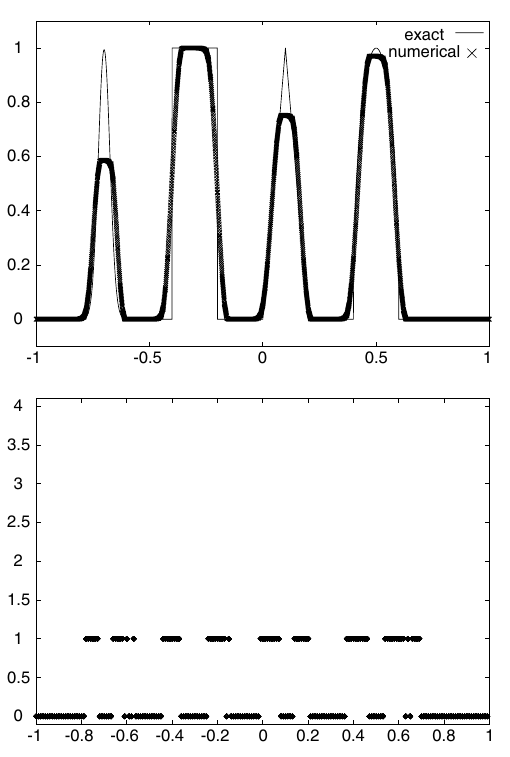
\includegraphics[width=\textwidth]{figures/moment-p-1}
    \caption{$p = 1$, moment limiter reduced to $\minmod$}
    \label{fig:results-advection-p1}
  \end{subfigure}
  \hfill
  \begin{subfigure}[t]{0.48\columnwidth}
    \centering
    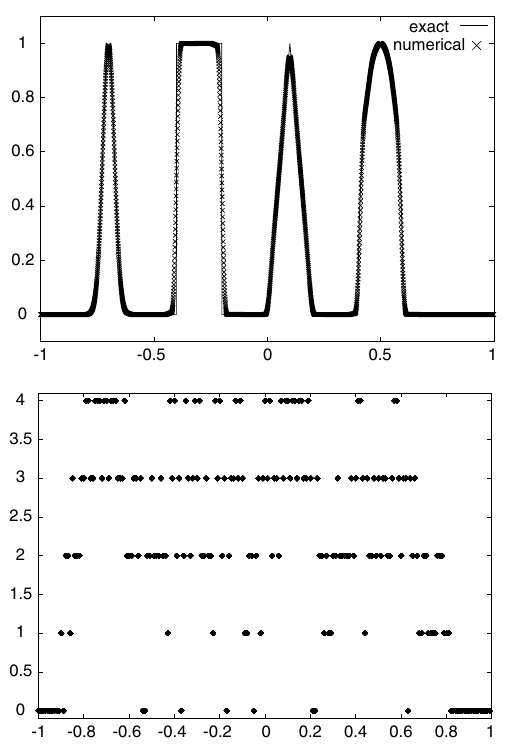
\includegraphics[width=\textwidth]{figures/moment-p-4}
    \caption{$p = 4$, with full moment limiter}
    \label{fig:results-advection-p4}
  \end{subfigure}
  \caption{Linear advection of various shapes on $200$ cells. Top part shows exact and numerical solutions while bottom part shows limiter activity. \cite[figure 2]{Krivodonova}}
  \label{fig:results-advection}
\end{figure}

The results are displayed in figure \ref{fig:results-advection}.
Figure \ref{fig:results-advection-p1} shows the results for $p = 1$ and figure \ref{fig:results-advection-p4} shows the results for $p = 4$, whereas in both figures the top part is a plot of the current state and the bottom part indicates limiter activity.
A dot in the activity plot marks the highest coefficient that was not limited, e.g. a point at 2 means that coefficients $3$ and $4$ were limited.

In the case of $p = 1$ the moment limiter which is identical to $\minmod$ here, behaves as expected.
The discontinuities have been noticeably smeared and a good portion of the height of the sharp peaks has been limited away.
At the same time though any oscillations were successively prevented.
The results for the fourth-order polynomials -- and thus fourth-order moment limiter -- came out better by all accounts.
There is no loss of height visible for the Gaussian bell shape as well as the half-ellipse and it has been reduced for the triangle.
Furthermore the approximations to the discontinuities have remained steeper and the corners on the square pulse are less rounded.
It is important to see that these improvements did not arise from the increase in polynomial degree but from the fact that the moment limiter discards less information.
$\minmod$ applied to fourth degree polynomials would limit the result to a similar degree as shown in figure \ref{fig:results-advection-p1}.

The activity plots are not as easily digestible.
In the first-order case we see that the limiter is not active in areas where the exact solution has steep gradients.
So there the coefficients are naturally bounded by the first-order approximations.
Curiously, the limiter is active in the flat regions.
A possible explanation is that the DG solver erroneously produces polynomial coefficients for higher degrees on the order of machine precision which are then bounded by difference quotients that are truly equal to $0$.
For $p = 4$ the activity plot shows that all four levels of limiting are used across the domain.
Additionally it extends the phenomenon from the first case to higher-order case that the limiter is most aggressive in flat regions and most permissive in the vicinity of steep gradients.
